\documentclass[conference]{IEEEtran}
\IEEEoverridecommandlockouts
% The preceding line is only needed to identify funding in the first footnote. If that is unneeded, please comment it out.
\usepackage{cite}
\usepackage{amsmath,amssymb,amsfonts}
% \usepackage{algorithmic}
\usepackage{graphicx}
\usepackage{textcomp}
\usepackage{xcolor}
\def\BibTeX{{\rm B\kern-.05em{\sc i\kern-.025em b}\kern-.08em
    T\kern-.1667em\lower.7ex\hbox{E}\kern-.125emX}}


\usepackage{cite}
\usepackage{amsmath,amssymb,amsfonts}
% \usepackage{algorithmic}
\usepackage{graphicx}
%\usepackage{textcomp}
\usepackage{xcolor}
% \usepackage{ulem}
\usepackage{makecell}
\usepackage{booktabs} 
%\usepackage{subfigure}
\usepackage{subfig}
\usepackage{graphicx}
\usepackage{amsmath}
%\usepackage{color}
%\usepackage{amssymb}
%\usepackage{mathrsfs}
\usepackage[normalem]{ulem}
%\usepackage{geometry}
\usepackage{enumitem}
\usepackage{multirow}
%\usepackage[ruled,vlined]{algorithm2e}
%\usepackage{algorithm2e}
%\usepackage{ulem}
\usepackage[nomargin,inline,marginclue,draft]{fixme}
\usepackage{balance}
%\usepackage{verbatim}
%\usepackage{diagbox}
\usepackage{changepage}


% \usepackage[table,xcdraw]{xcolor}
\usepackage{balance}
\usepackage[breaklinks=true,bookmarks=false]{hyperref}
\newcommand{\para}[1]{{\vspace{1pt} \bf \noindent #1 \hspace{10pt}}}
\usepackage{fixme}
\fxsetup{status=draft}
\usepackage{multirow}
\usepackage{algorithm}
\usepackage{algpseudocode}

\usepackage{etoolbox}
\makeatletter
\patchcmd{\@makecaption}
  {\scshape}
  {}
  {}
  {}
\makeatother

\newcommand{\chen}[1]{\footnote{+chen+: #1}}


\begin{document}

\title{Session-aware Item-combination Recommendation with Transformer Network}
% *\\
% {\footnotesize \textsuperscript{*}Note: Sub-titles are not captured in Xplore and
% should not be used}
% \thanks{Identify applicable funding agency here. If none, delete this.}
% }

\author{\IEEEauthorblockN{Tzu-Heng Lin}
\IEEEauthorblockA{
% \textit{dept. name of organization (of Aff.)} \\
\textit{Peking University}\\
lzhbrian@gmail.com}
\and
\IEEEauthorblockN{Chen Gao}
\IEEEauthorblockA{
\textit{Department of Electronic Engineering} \\
\textit{Tsinghua University}\\
chgao96@gmail.com}
}



\maketitle

\begin{abstract}
    In this paper, we detailedly describe our solution for the IEEE BigData Cup 2021: RL-based RecSys (Track 1: Item Combination Prediction)\footnote{https://www.kaggle.com/c/bigdata2021-rl-recsys/}.
    We first conduct an exploratory data analysis on the dataset and then utilize the findings to design our framework.
    Specifically, we use a \textbf{two-headed transformer-based network} to predict user feedback and unlocked sessions, along with the proposed \textbf{session-aware reweighted loss}, \textbf{multi-tasking with click behavior prediction}, and \textbf{randomness-in-session augmentation}.
%   \chen{we can use two-three sentences to describe our method. It would be better if we can name it.}
    In the final private leaderboard on Kaggle, our method ranked 2nd with a categorization accuracy of 0.39224.\footnote{Our code is available at https://github.com/lzhbrian/bigdatacup2021}
\end{abstract}

\begin{IEEEkeywords}
recommender system, item combination prediction, transformer, loss reweighting
\end{IEEEkeywords}


% intro


\section{Introduction} \label{sec:intro}



The task of the IEEE BigData Cup 2021: RL-based RecSys (Track 1: Item Combination Prediction) \cite{2021RL4RS, kaggle} is to predict each user's purchasing feedback to nine exposed items, given this user's click history, portrait features, and items' features, which is similar to \textit{bundle recommendation}~\cite{chang2020bundle}.
The special setting in this task is that the nine items are grouped into three sessions. 
The user can only unlock the subsequent session after he/she buys all three items in the current session.

More formally, given a user $u$ (along with his/her clicking history $c_{u,1}, c_{u,2}, ...$, and some portrait features $f_{u,1}, f_{u,2}, ..., f_{u,10}$), and his/her nine exposed items $i_{u,1}, i_{u,2}, ..., i_{u,9}$ (along with some item features $f_{i,1}, f_{i,2}, ..., f_{i,6}$ for each item $i$), 
the objective is to predict nine interactions $y_{u,1}, y_{u,2}, ..., y_{u,9} \in \{0,1\}$.
Each one of the interactions indicates whether this user would buy the corresponding item or not. 
In addition, in this scenario, the middle three items $i_{u,4}, i_{u,5}, i_{u,6}$ are not unlocked until the user has bought all of the first three items $i_{u,1}, i_{u,2}, i_{u,3}$, and similarly, the last three items $i_{u,7}, i_{u,8}, i_{u,9}$ are not unlocked until the user has bought all of the first six items $i_{u,1}, i_{u,2}, ..., i_{u,6}$ (\textit{c.f.} Figure \ref{fig:problemdef}). 
% metric
The evaluation metric for this task is the Categorization Accuracy measure, which is defined as follows,
\begin{equation}
    \textbf{accuracy} = \frac{1}{M} 
    ~\overset{M}{\underset{u=1}{\sum}}  ~\overset{9}{\underset{j=1}{\prod}} 
    ~[y_{u,j} = \hat{y}_{u,j}],
\end{equation}
where $M$ denotes the number of users, $y_{u,j}$ and $\hat{y}_{u,j}$ are the predicted and ground-truth interactions, and $[y_{u,j} = \hat{y}_{u,j}]$ is the \textit{Iverson bracket}.

% challenging
Overall speaking, this task is challenging in two aspects.
\begin{itemize}
    \item Firstly, the nine exposed items are correlated and treated differently by the users. We cannot simply apply a single traditional recommendation method to predict each interaction independently.
    \item Secondly, with the given evaluation metric, it is required to correctly predict all of the nine interactions of a user, while partially correct predictions contribute nothing to the final score.
\end{itemize}
%

% \begin{table}[t!]
%     \centering
%     \caption{Private Leaderboard on Kaggle}
%     \begin{tabular}{c|c|c}
%         rank & team name & score \\\hline
%         1 & lovers (AIN and HGRU) & 0.42069 \\\hline
%         \textbf{2} & \textbf{lzhbrian (ours)} & \textbf{0.39224} \\\hline
%         3 & Tom\&Jerry (LightGBM) & 0.39157 \\
%     \end{tabular}
%     \label{tab:lb}
% \end{table}

\begin{figure}[t!]
    \centering
    \includegraphics[width=\linewidth]{figures/problemdef.pdf}
    \caption{Problem Setup. Each user is exposed to nine items simultaneously. However, the items are divided into three 3-length sessions. The user can only unlock the subsequent three items after he/she buys all three items in the current session.
    We want to predict whether a user would buy the nine exposed items or not.}
    \label{fig:problemdef}
\end{figure}


\IEEEpubidadjcol

To overcome the above challenges, we propose a delicate two-headed transformer-based framework to predict both users' buying behavior and unlocked sessions.
The unlocked session prediction can be used to refine unreasonable buy predictions.
We further propose a randomness-in-session augmentation technique and a novel session-aware reweighted loss to address the unique characteristics in this scenario.
Finally, a multi-tasking training procedure with click prediction is utilized to assist the learning of embedding layers.
Extensive experiments and ablation studies have demonstrated the effectiveness of our method.

% following
In what follows, we will discuss related works in Section \ref{sec:relatedwork}, conduct an exploratory data analysis in Section \ref{sec:eda}, describe our proposed method in Section \ref{sec:method}, and finally conclude the paper with discussion and future works in Section \ref{sec:conclusion}.

% \chen{input and output}




% EDA
\section{Exploratory Data Analysis} \label{sec:eda}
Before diving into the model design, we conduct exploratory data analysis firsthand to master the whole picture of the dataset.

\subsection{Data statistics}
Table \ref{tab:datastats} shows the overall statistics of this dataset. 
In total, there are 381 items.
There are 260,087 buying entries for training and 206,254 buying entries for testing. These entries are also accompanied by 10,435,798 and 8,357,719 clicking logs, respectively. We will then analyze more details about the clicking and buying behavior of users in the following.

\begin{table}[t!]
    \centering
    \caption{Overall data statistics}
    \begin{tabular}{c|c|c|c|c}
        \hline
        \multicolumn{2}{c|}{\# buying entries (users)} &
        \multicolumn{2}{c|}{\# clicks} &
        \multirow{2}{*}{\# items} \\
        \cline{1-4}
          \# train & \# test & \# train & \# test & \\
        \hline
        260,087 & 206,254 & 10,435,798 & 8,357,719 & 381 \\
        \hline
        \end{tabular}
    \label{tab:datastats}
\end{table}

Table \ref{tab:clickbuysess} shows how many clicks and buys do items in each session possess. It's worth noticing that an item would only appear in its specific session.
We can see that items in later sessions are with more types, and items with earlier sessions possess more clicks and buys. This is reasonable since users need to buy early items in order to unlock items (with higher prices) in the later sessions.


\begin{table}[t!]
    \centering
    \caption{Click and buy statistics in different sessions.}
    \begin{tabular}{c|c|c|c|c} 
    \hline
    {session} & {item IDs} & {\# items} & {\# clicks} & {\# buys} \\ \hline
    {1} & {1$\sim$39}& 39 & {4,606,977} & {616,952} \\ \hline
    {2} & {40$\sim$147} & 108 & {3,608,173} & {485,449} \\ \hline
    {3} & {148$\sim$381} & 234 & {2,220,648} & {287,482} \\ \hline
    \end{tabular}
    \label{tab:clickbuysess}
\end{table}


\subsection{Buying behavior analysis} \label{sec:eda:buyanalysis}
Due to the dataset characteristics (\textit{c.f.} Section \ref{sec:intro}), we plot the histogram of the number of items each user bought in Fig. \ref{fig:analysis:buy}, and classify users into four groups according to the number of items they have bought as follows,
\begin{itemize}
    \item Group-0: 30,912 users who have bought 0 item.
    \item Group-1: 50,267 users who have bought 1$\sim$3 items.
    \item Group-2: 38,191 users who have bought 4$\sim$6 items.
    \item Group-3: 140,717 users who have bought 7$\sim$9 items.
\end{itemize}
We can see that a decent population (Group-0) didn't buy anything, the number of users who bought 4$\sim$6 items (Group-2) are the fewest, and a large portion of users (Group-3) chose to buy no less than seven items. This indicates an \textbf{hourglass shape of user distribution}.
It's also worth noticing that very few people buy three or six items (\textit{c.f.} Fig. \ref{fig:analysis:buy}). We hypothesize that this is because the main reason why a user buys three or six items is to unlock and buy items in the next session.

\begin{figure}[t!]
    \centering
    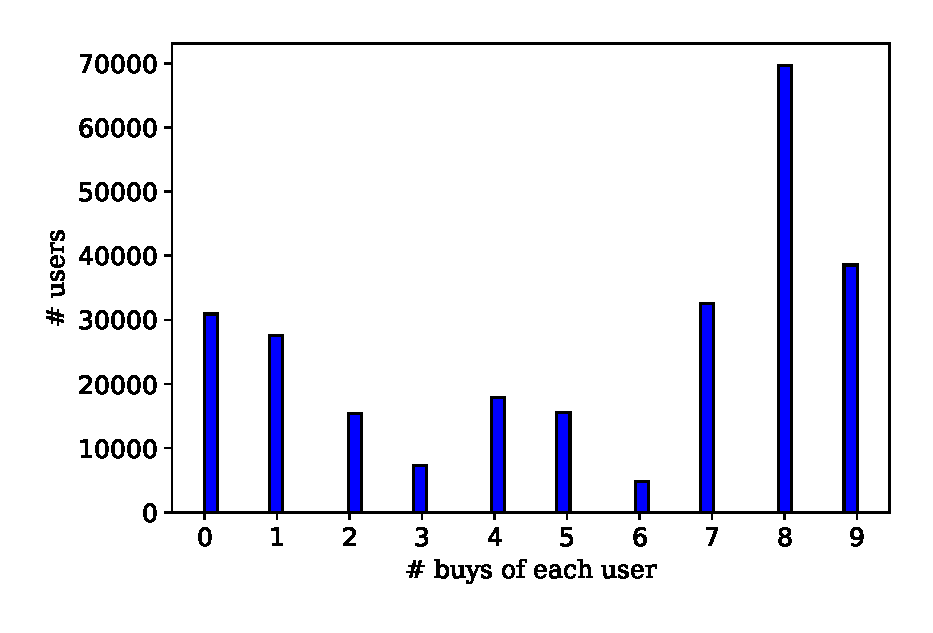
\includegraphics[width=0.8\linewidth]{figures/analysis/buy.eps}
    \caption{Histogram of the number of buys of each user.}
    \label{fig:analysis:buy}
\end{figure}


% click
\subsection{Clicking behavior analysis} 
We plot the histogram of the number of clicks of each user in Fig. \ref{fig:analysis:click}.
There are 28,184 users who did not click anything. However, we do see that the majority of users are with a decent number of clicks, which motivates us to utilize the clicking logs to assist the training.

% buy
\begin{figure}[t!]
    \centering
    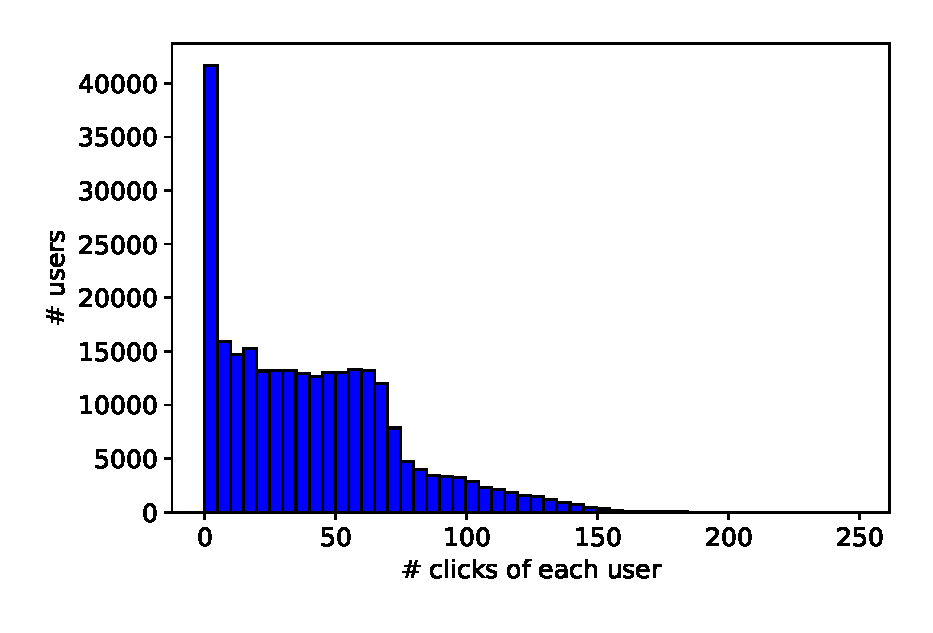
\includegraphics[width=0.8\linewidth]{figures/analysis/click.eps}
    \caption{Histogram of the number of clicks of each user.}
    \label{fig:analysis:click}
\end{figure}


\subsection{User portrait features and item features}
We further present user portrait features and item features in Table \ref{tab:user_portrait} and Table \ref{tab:item_features}.
We can see that all user portraits are discrete features, while two of the item features are continuous features.

\begin{table*}[t!]
    \centering
    \caption{User portrait features.}
    \begin{tabular}{c|c|c|c|c|c|c|c|c|c|c}
    \hline
    {\textbf{user features}} & 
    { $f_{u,1}$} & 
    { $f_{u,2}$} & 
    { $f_{u,3}$} & 
    { $f_{u,4}$} & 
    { $f_{u,5}$} & 
    { $f_{u,6}$} & 
    { $f_{u,7}$} & 
    { $f_{u,8}$} & 
    { $f_{u,9}$} & 
    { $f_{u,10}$} \\ \hline
    { \# unique values in train set} & 3 & { 1363} & { 20} & { 10} & { 195} & { 49} & { 3} & { 11} & { 2} & { 2164} \\ \hline
    { \# unique values in test set} & 3 & { 1319} & { 19} & { 10} & { 191} & { 47} & { 3} & { 13} & { 2} & { 2054} \\ \hline
    %{ \# unique values in testset\_track2} & 3 & { 1341} & { 20} & { 10} & { 190} & { 47} & { 3} & { 11} & { 2} & { 2060} \\ \hline
    discrete or continuous (disc./cont.) & disc. & disc. & disc. & disc. & disc. & disc. & disc. & disc. & disc. & disc. \\ \hline
    \end{tabular}
    \label{tab:user_portrait}
\end{table*}



\begin{table*}[t!]
    \centering
    \caption{Item features.}
    \begin{tabular}{c|c|c|c|c|c|c}
    \hline
    { \textbf{item features}} & { $f_{i,1}$} & 
    { $f_{i,2}$} & 
    { $f_{i,3}$} & 
    { $f_{i,4}$} & 
    { $f_{i,5}$} & 
    { $f_{i,6}$ (price)} \\ \hline
    {\# unique values} & {4} & {10} & {2} & {n/a} & {n/a} & {248} \\ \hline
    % \rowcolor[HTML]{333333} 
    {values} & {1,2,3,4} & {0,1,2,3,4,5,6,7,8,9} & {1,2} & { 0$\sim$1, float} & {0$\sim$1, float} & {150$\sim$16621, int} \\ \hline
    discrete or continuous (disc./cont.) & disc. & disc. & disc. & cont. & cont. & cont. \\ \hline
    \end{tabular}
    \label{tab:item_features}
\end{table*}



% \chen{it seems that we have not summarized the conclusions of the EDA}

% method
\section{Method} \label{sec:method}

% \begin{figure*}[!h]
%     \centering
%     \includegraphics[width=\linewidth]{figures/net.png}
%     \caption{Overall structure of our method.}
%     \label{fig:net}
% \end{figure*}
\begin{figure*}[t!]
    \centering
    \includegraphics[width=0.5\linewidth]{figures/reweightloss.png}
    \caption{Session-Aware Loss Reweighting}
    \label{fig:reweightloss}
\end{figure*}

The overall structure of our method is shown in Figure \ref{fig:net}. 
In what follows, we will introduce each of our designs respectively.


%%%%%%%%%%%%%%%%%%%%%%%%%%
% two head
\subsection{Two-headed (Buy and Session) Prediction} \label{sec:method:twohead}
% \chen{1.to improve it, we can provide formulations rather than only texts; 2. to explain the motivations of each design}
We start with a two-headed prediction structure (Figure \ref{fig:net} left).
The network takes the following inputs: user profile features, user clicked items' id and features, 9 exposed target items' id and features.
%
These inputs are further processed by their corresponding embedding layers, and a backbone network (\textit{e.g.} MLP).
%
Finally, the network predicts whether the user will buy the 9 exposed target items or not, and to which session (\textit{c.f.} Section \ref{sec:eda:stats}) will the user unlock.
%
The predicted session will be used to refine the predicted results of the 9 exposed target items.

% design motivation
We design this framework for the following reasons:
%
Firstly, the 9 item feedbacks are correlated. For example, users might buy all of the first 6 items, only to buy the 9th item. It is not suitable to predict the 9 feedbacks independently. So we design a network that is able to predict 9 feedbacks simultaneously.
%
Secondly, if we only predict the 9 feedbacks, there might be mistakes where the predicted results are impossible to happen in the real world. For example, the network might predict one only buys the 1st and the 9th items. This is impossible since the user has to buy all of the first 6 items, in order to buy the 9th item. So we design another head to predict the unlocked sessions of users. The results are used to fix unreasonable outputs of the buy feedback predictions.



%%%%%%%%%%%%%%%%%%%%%%%%%%
% reweight
\subsection{Session-Aware Loss Reweighting}


To better model users' buy behaviors, we classify the 9 exposed items into 4 categories according to each user's buy behavior (weak positive, strong positive, strong negative, weak negative) as shown in Figure \ref{fig:reweightloss}.
%
For sessions before the last session user has unlocked, items should be treated as weak positives, as user might buy these items only to unlock the later sessions.
%
For the last session user has unlocked, items should be treated as strong positives and strong negatives. As user unlocked and stopped in this session, items bought or not bought should be classified as strong signals.
%
For later locked sessions, items should be treated as weak negatives, as users haven't unlocked these sessions, we shouldn't assume too strong preference on these items.

In practice, we reweight the BCE loss of these 4 categories using weight 0.5, 1, 1, 0.5, respectively.
In our experiments, reweighting loss provide huge improvements to the final score (from 0.365 to 0.388).


%%%%%%%%%%%%%%%%%%%%%%%%%%
% multitask click
\subsection{Multi-tasking with Click Behavior Prediction}
Apart from the network described in \ref{sec:method:twohead}, we use another network to predict user click behavior (Figure \ref{fig:net} right).
The two networks share the same embedding layers.
We argue that through this multi-tasking procedure, the embedding layers can be better learned.
%
In our early ablation study, this can improve our score from 0.362 to 0.365.


%%%%%%%%%%%%%%%%%%%%%%%%%%
% transformer
\subsection{Transformer Backbone}
Instead of simple MLPs \cite{din, ncf}, we switch the backbone part of buy behavior prediction and click behavior prediction into transformers \cite{transformer}, as their self-attention mechanism is proved to be effective on capturing inter-relations between different features.
%
In our early ablation study, this can improve our score from 0.36 to 0.365.




%%%%%%%%%%%%%%%%%%%%%%%%%%
% aug, tta
\subsection{Randomness-in-session Augmentation}
To prevent over-fitting and make training more robust, we randomly shuffle items' order within the same sessions. 
This strategy is also used for test time augmentation, where orginal prediction and shuffled predictions are averaged to produce the final results.
In our experiments, augmentation in training provides minor difference, while augmentation in testing provides an unstable improvement of around 0.002.



%%%%%%%%%%%%%%%%%%%%%%%%%%
\subsection{Other settings}
Colab with a P100 GPU is used as our training platform.
We use Adam \cite{adam} with default hyper-parameters in PyTorch \cite {pytorch}.
Batch size is set to 32, and learning rate is set to 1e-2 for 10 epochs, and 1e-3 for another 10 epochs.
%
Clicking data in the test set of both tracks is also used during our training. 
%
All continuous features are discretized into bins (including item features, prices).




% \newpage
% things
% \input{4.things}

% discussion
\section{Conclusion} \label{sec:conclusion}


% \subsection{Discussion}
In this paper, we propose a framework for item combination prediction. Specifically, we propose several delicate designs to improve the performance, namely randomness-in-session augmentation, transformer backbone, two-headed prediction, session-aware loss reweighting, and multi-tasking with click prediction.
Extensive experiments have proved the effectiveness of our framework.

%% Thing didn't work
We have also tried several things that conceptually make sense but did not improve the score.
% DIN
Firstly, we tried an attention-like deep interest network \cite{din} to reweight user clicked items, but however, it didn't improve the final score.
Given that we do not know how click data is collected, we think that users might present different preferences in the scenario where click data is collected. And thus, making the model more complex in this aspect doesn't help.
% user emb
Secondly, we tried to add user embedding into the network yet encountered severe over-fitting in training. Adding mini-batch aware regularization \cite{din} can reduce over-fitting, but however, it still cannot make improvements to the final score.
Due to the fact that most users only have one training entry, this result is not very surprising.
% Timestamp embedding
In addition, we tried adding timestamp as a feature, but however, it also didn't help. We originally thought that weekends or holidays might affect user behaviors.


% \chen{we can explain the above results}

% future work
Future works shall include in-depth analysis and utilization with the actual meaning of user features, item features, and clicking data. It would also be interesting to investigate other network architectures that could address the multi-feedback item combination prediction scenario.
Since our work does not introduce the model ensemble technique, it is also a promising direction for future works.


% \newpage

\balance
\bibliographystyle{IEEEtran}
\bibliography{ref}



\end{document}
